%
% main.tex -- Paper zum Thema <aircraft>
%
% (c) 2026 Stephanie Märklin, OST Ostschweizer Fachhochschule
%
% !TEX root = ../../buch.tex
% !TEX encoding = UTF-8
%
\chapter{Komplexe Eigenwerte in der Flugdynamik\label{chapter:aircraft}}
\kopflinks{Komplexe Eigenwerte in der Flugdynamik}
\begin{refsection}
\chapterauthor{Stephanie Märklin}

Im Flug ist ein Flugzeug ständigen Störungen ausgesetzt, die seine
Lage verändern.
Wie ein Flugzeug auf Störungen antwortet, ist eine grundlegende
Eigenschaft des Flugzeugs.

Welche Antwort erwünscht ist, hängt vom Zweck ab.
Ein einmotoriges Schulflugzeug soll nach einer Störung idealerweise von selbst
in die ursprüngliche Lage zurückkehren.
Dieses Verhalten erleichtert es dem Piloten, das Flugzeug sicher zu
steuern.
Man nennt ein solches Flugzeug stabil.
Ein moderner Kampfjet ist bewusst instabil gebaut, um ein
Maximum an Agilität zu erreichen.
Fliegbar bleibt er nur, weil Computersysteme ihn in jedem Augenblick
stabilisieren

Ob stabil oder bewusst instabil, die Eigenschaft steckt in der
Konstruktion und steht fest, bevor das Flugzeug zum ersten Mal
fliegt.
Der Flugversuch kommt als Nachweis also zu spät.
Die Stabilität muss vorher berechnet werden.
Dieses Kapitel zeigt, wie sich die Bewegung des Flugzeugs als
Differentialgleichung schreiben lässt.
Ihre Lösung drückt die Stabilität in wenigen Zahlen aus.

\input{papers/aircraft/0-motivation.tex}
% (c) 2026 Stephanie Märklin, OST Ostschweizer Fachhochschule
%
% !TEX root = ../../buch.tex
% !TEX encoding = UTF-8
%
% Rolle im Paper: Konkretisierung des Problems. Das allgemeine Problem auf
% einen konkreten,% behandelbaren Fall eingrenzen und die Wahl begründen
%
% Stichworte:
% 17.1 Grundbegriffe
% - welche Begriffe folgen und wozu (Werkzeugkasten für die Leitfrage)
% - Achsen benennen: Rollen/Längsachse, Nicken/Querachse, Gieren/Hochachse
% - Ruhelage konkret: getrimmter Geradeausflug; Störung: Böe
% - Definition stabil: selbständige Rückkehr, ohne Piloteneingriff
%   (stick fixed), auf allen drei Achsen
%
% 17.1.1 Stabilität
% - Kernpunkt: Stabilität ist eine Eigenschaft des Flugzeugs selbst --
%   sie entsteht durch die Konstruktion (Geometrie, Leitwerk) und
%   bestimmt Einsatz und Handhabung
% - Anknüpfen: Definition aus 17.1 ist qualitativ (stabil ja/nein)
% - Konkretisierung: ja/nein nicht genug für die Eigenschaft
%   wir müssen wissen OB und WIE schnell die Bewegung abklingt
% - Problem: Erfliegen/Beobachten liefert die Antwort erst, wenn das
%   Flugzeug existiert, das ist zu spät
% - Folgerung: wir müssen die Bewegung nach der Störung berechnen können
%   (Leitfrage konkretisiert)
% - Übergang: dazu braucht es eine mathematische Beschreibung der
%   Bewegung -> Aufzeigen anhand der Dutchroll (führt zu 17.1.2)

% Stichworte:
% 17.1.2 Die Dutch Roll
% - Phänomen beschreiben: Nase schwingt links-rechts, Flügel wippen
%   gegenphasig (Verweis auf Abbildung?)
% - Mechanismus verbal als Kreislauf: Gieren erzeugt Schieben,
%   Schieben erzeugt Rollen, Rollen erzeugt Gieren
% - dabei: Schieben ist NEU -- keine Drehbewegung, sondern seitliche
%   Bewegung; kurz einführen (ein Satz), formal als Schiebewinkel
%   erst in 17.2
% - Pointe: die Bewegungen sind gekoppelt -- keine Achse lässt sich
%   allein betrachten
% - Schluss (Übergang): ob die Schwingung abklingt und wie schnell,
%   lässt sich am Phänomen nicht ablesen -- dafür brauchen wir die
%   Grössen, die die Bewegung beschreiben (-> 17.2)

\section{Grundbegriffe der Flugstabilität
\label{aircraft:section:1-grundbegriffe}}
\kopfrechts{Grundbegriffe}
Um die Stabilität eines Flugzeugs beschreiben zu können, führen wir zunächst
die drei Flugzeugachsen und ihre Drehbewegungen ein.
Die Abbildung~\ref{aircraft:fig:achsen} zeigt die drei Achsen mit den
zugehörigen Drehbewegungen.
Das \emph{Nicken} (pitch) ist die Drehbewegung um die Querachse, das
\emph{Rollen} (roll) die Drehbewegung um die Längsachse und das \emph{Gieren}
(yaw) die Drehbewegung um die Hochachse.
\input{papers/aircraft/fig/fig-achsen}
Als Ruhelage betrachten wir den getrimmten Geradeausflug:
Die Flügel liegen horizontal, das Flugzeug nickt und giert nicht.
Eine Störung wie eine Böe bewegt das Flugzeug aus der Ruhelage.
Das Flugzeug heisst stabil, wenn es ohne Eingriff des Piloten in die
Ruhelage zurückkehrt.

\subsection{Stabilität als Flugzeugeigenschaft
\label{aircraft:subsection:eigenschaft}}
Die Stabilität ist eine Eigenschaft des Flugzeugs selbst.
Sie beeinflusst unter anderem dessen Handhabung und Agilität.
Bestimmt wird sie durch die Konstruktion und damit bereits im Entwurf.

Die Definition aus Abschnitt~\ref{aircraft:section:1-grundbegriffe}
beurteilt die Stabilität nur qualitativ.
Das Flugzeug kehrt in die Ruhelage zurück oder nicht.
Für die Konstruktion müssen wir wissen, ob das Flugzeug zurückkehrt und wie
schnell die Bewegung abklingt.
Die Ermittlung durch Messungen liefert diese Antwort erst, wenn das
Flugzeug gebaut ist, und damit zu spät für den Entwurf.
Wir müssen die Bewegung nach einer Störung bereits vorher berechnen können.
Welche Grössen diese Bewegung beschreiben, zeigt sich an einem Phänomen,
bei dem sich die Drehbewegungen gegenseitig beeinflussen: der Dutch Roll.

\subsection{Die Dutch Roll
\label{aircraft:subsection:dutchroll}}
Die \emph{Dutch Roll} ist ein charakteristisches Schwingungsmuster.
Die Abbildung~\ref{aircraft:fig:dutchroll} zeigt ihren Ablauf.
%! Author = stephaniemaerklin
%! Date = 30.08.2026

\begin{figure}
    \centering
    \includegraphics[width=0.7\textwidth]{papers/aircraft/images/dutchroll.png}
    \caption{Ablauf der Dutch Roll.
    Oben die Vorderansicht, das Flugzeug rollt abwechselnd nach rechts und
    nach links, die punktierte Linie ist die Flugbahn.
    Unten die Draufsicht, das Flugzeug fliegt von rechts nach links, die Nase
    pendelt um die Flugrichtung, das Flugzeug giert und schiebt.
    \label{aircraft:fig:dutchroll}}
\end{figure}
Eine Störung dreht die Nase nach links (1).
Der rechte Flügel senkt sich (2), und die Nase dreht zurück nach
rechts (3).
Darauf senkt sich der linke Flügel (4), und die Nase dreht erneut
nach links (5).
Das Flugzeug überschiesst die Ruhelage.
Es entsteht eine Schwingung.
In den Drehbewegungen ausgedrückt heisst das:
Gieren erzeugt Schieben, Schieben erzeugt Rollen, und Rollen erzeugt
erneut Gieren.
Dabei bezeichnet \emph{Schieben} (sideslip), dass die Bewegungsrichtung des
Flugzeugs von seiner Längsachse abweicht.

% QR-CODE 1 (Herausgeber): rechts neben diesem Absatz
% Ziel: https://www.youtube.com/watch?v=9Gt-IcCBiQ4
% Beschriftung: Vorschlag "Video: Erklärung Dutch Roll (en)"
%
% videoqrcode.tex
%
% (c) 2026 Prof Dr Andreas Müller
%
\vspace*{-12pt}
\smash{\hbox to12.26cm{\hfill\raisebox{-2.2cm}{%
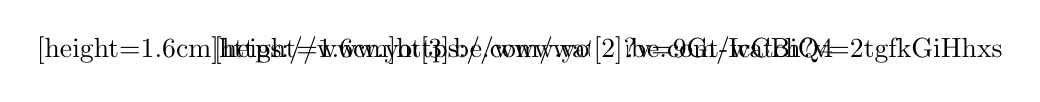
\begin{tikzpicture}
\node at (-1.1,0) {\qrcode[height=1.6cm]{https://www.youtube.com/watch?v=9Gt-IcCBiQ4}};
\fill[color=white] (-1.1,0) circle[radius=0.24];
\node at (-1.1,0) {[3]};
\node at (1.1,0) {\qrcode[height=1.6cm]{https://www.youtube.com/watch?v=2tgfkGiHhxs}};
\fill[color=white] (1.1,0) circle[radius=0.24];
\node at (1.1,0) {[2]};
\end{tikzpicture}
}}}%
\hangindent=-4.4cm
\hangafter=-6

\phantom{000}Das Video \cite{aircraft:video-erklaerung} zeigt diesen Ablauf in Bewegung.
Es erklärt zusätzlich, welche Eigenschaften des Flugzeugs die Schwingung
begünstigen; darauf kommen wir in Abschnitt 17.7 zurück.
%
%
% QR-CODE 2 (Herausgeber): rechts neben diesem Absatz
% Ziel: https://www.youtube.com/watch?v=2tgfkGiHhxs
% Beschriftung: Vorschlag "Video: Aufnahme Dutch Roll"
Wie intensiv eine Dutch Roll ausfallen kann, zeigt die Aufnahme
\cite{aircraft:video-aufnahme} eines dreistrahligen Verkehrsflugzeugs.

Die Dutch Roll ist eine von drei Bewegungsformen, mit denen ein
Flugzeug auf eine Störung der \emph{Seitenbewegung} (lateral motion) antwortet.
Die Seitenbewegung umfasst das Gieren, das Schieben und das Rollen.
Die \emph{Rollbewegung} (roll mode) ist eine Drehung um die Längsachse.
Der absinkende Flügel erzeugt dabei mehr Auftrieb als der steigende und bremst
die Drehung.
Bei gewöhnlichen Anstellwinkeln klingt die Rollbewegung deshalb rasch ab.
Die \emph{Spiralbewegung} (spiral mode) verläuft ohne Schwingung.
Das Flugzeug neigt sich langsam zur Seite, die Nase dreht in die Kurve, und der
Rollwinkel wächst weiter.
Ob die Spiralbewegung abklingt oder anwächst, hängt von der Konstruktion ab.
In beiden Fällen ist die Bewegung so langsam, dass der Pilot sie leicht
korrigieren kann.
Die Dutch Roll dagegen ist eine Schwingung, bei der offen bleibt, ob sie
abklingt und wie schnell.
Im Folgenden untersuchen wir deshalb die Dutch Roll.

Ob die Schwingung abklingt und wie schnell, lässt sich am Schwingungsmuster
nicht direkt ablesen.
Dafür brauchen wir Grössen, die die Bewegung beschreiben.

% (c) 2026 Stephanie Märklin, OST Ostschweizer Fachhochschule
%
% !TEX root = ../../buch.tex
% !TEX encoding = UTF-8
%
% Rolle im Paper: Realität in ein mathematisches Objekt übersetzen;
% Annahmen benennen
%
% Stichworte:
% 17.2 Das Flugzeug als dynamisches System (Vorspann, unnummeriert)
% - Ziel: Flugzeug -> dynamisches System übersetzen; Begriff einführen
%   (mathematisches Objekt, dessen Zustand sich mit der Zeit ändert)
% - Begriffe aus 17.1 beschreiben nur die Lage; Erweiterung um
%   Grössen, die die Bewegung erfassen
% - Beschränkung: Seitenbewegung (lateral motion) = Gieren, Schieben,
%   Rollen -- nur diese sind an der Dutch Roll beteiligt
% - Annahme: Störung klein, Betrachtung nahe der Ruhelage
% - Fahrplan am Ende ("Für diese Übersetzung ..."): Zustandsvektor ->
%   Bewegungsgesetz -> Systemmatrix

% 17.2.1 Der Zustandsvektor der Seitenbewegung
% - vier Grössen einzeln: Schiebewinkel beta (formalisiert das
%   Schieben aus 17.1.2), Rollrate p, Gierrate r, Rollwinkel phi
% - Tabelle: Symbol, Name, Bedeutung
% - Notation nach Nelson \cite (ein Satz, deckt die Tabelle ab)
% - Zustandsvektor x = [beta, p, r, phi]^T (equation, Label)
% - ein Satz Rückgriff: beta verbindet Gieren und Rollen;
%   Konsequenz folgt in Abschnitt 17.4 (Vorverweis, kein Vorgriff)
% - Schluss (Paar, keine Überleitung): x = Momentaufnahme zur Zeit t;
%   Ableitung xdot beschreibt, wie sich der Zustand verändert

% 17.2.2 Das Bewegungsgesetz
% - Andocken: wir suchen den Zusammenhang zwischen x und xdot
% - für kleine Störungen um die Ruhelage linear -> xdot = Ax
%   (equation, Label); \emph{Systemmatrix} benennen;
%   Herleitung: Nelson \cite
% - Gleichung lesen: Änderung jeder Zustandsgrösse ist eine
%   Linearkombination der momentanen Zustandsgrössen; A enthält
%   die Koeffizienten

% 17.2.3 Die Systemmatrix
% - Andocken: "Für die Seitenbewegung lautet die Systemmatrix ..."
% - A vollständig (equation, Label; exakt die Vortrags-Fassung)
% - neue Symbole erklären: g Erdbeschleunigung, V Fluggeschwindigkeit
% - offener Punkt: Schreibweise ggü. Nelson Gl. 5.33 vereinfacht --
%   Halbsatz ergänzen oder Konvention mit Formelskelett/MATLAB klären
% - zwei Zeilen vorlesen: pdot = Lbeta*beta + Lp*p + Lr*r (gehaltvoll)
%   und phidot = p (Buchhaltung; löst Rollen/Rollrate/Rollwinkel ein)
% - Einträge = aerodynamische Derivative; EIN Beispiel: Lbeta =
%   Rollmoment durch Schieben + Böen-Analogie (noch von Stephanie)
% - Struktur fix, Werte flugzeug-/flugzustandsspezifisch
%   (Tabelliert-Halbsatz gestrichen)
% - Schluss (Feststellung): "Damit ist das Flugzeug in ein
%   dynamisches System übersetzt."


\section{Das Flugzeug als dynamisches System
\label{aircraft:section:system}}
\kopfrechts{Dynamisches System}
Um die Bewegung nach einer Störung berechnen zu können, übersetzen wir
das Flugzeug in diesem Abschnitt in ein \emph{dynamisches System}.
Ein dynamisches System ist ein mathematisches Objekt, dessen Zustand sich mit
der Zeit verändert.
Dazu führen wir zuerst den Zustandsvektor ein, dann das
Bewegungsgesetz, das seine Änderung bestimmt, und die Systemmatrix mit ihren
Einträgen.

Wir beschränken uns dabei auf die Seitenbewegung.
Wir nehmen an, dass die Störung klein ist, und betrachten die
Bewegung in der Nähe der Ruhelage.

\subsection{Der Zustandsvektor der Seitenbewegung
\label{aircraft:subsection:zustandsvektor}}
Der Zustand ist die Momentaufnahme der Bewegung.
Für die Seitenbewegung genügen dazu vier Grössen.
Der \emph{Schiebewinkel} $\beta$ formalisiert das Schieben aus
Abschnitt~\ref{aircraft:subsection:dutchroll}:
Er misst den Winkel zwischen der Längsachse und der tatsächlichen
Bewegungsrichtung des Flugzeugs.
Die \emph{Rollrate} $p$ und die \emph{Gierrate} $r$ sind die
Änderungsraten des Rollens und des Gierens.
Der \emph{Rollwinkel} $\varphi$ misst die Drehung um die Längsachse
gegenüber der Ruhelage.
Wir folgen dabei der Notation von Nelson~\cite{aircraft:nelson}, der
die Seitenbewegung mit denselben Grössen beschreibt.

Wir fassen die vier Grössen zum \emph{Zustandsvektor}
\begin{equation}
    \vec{x}(t)
    =
    \begin{pmatrix}
        \beta(t) \\ p(t) \\ r(t) \\ \varphi(t)
    \end{pmatrix}
    \label{aircraft:eqn:zustandsvektor}
\end{equation}
zusammen.
Der Zustandsvektor ist die Momentaufnahme der Bewegung zur Zeit $t$.
Seine Ableitung $\dot{\vec{x}}(t)$ beschreibt, wie sich der Zustand
verändert.
% // TODO Referenz anpassen oder evtl. ganz streichen

\subsection{Das Bewegungsgesetz
\label{aircraft:subsection:bewegungsgesetz}}
Wir suchen den Zusammenhang zwischen dem Zustand $\vec{x}$ und seiner
Änderung $\dot{\vec{x}}$.
Für kleine Störungen um die Ruhelage ist dieser Zusammenhang linear
und es gilt
\begin{equation}
    \dot{\vec{x}}
    =
    A\vec{x}
    \label{aircraft:eqn:bewegungsgesetz}
\end{equation}
mit einer Matrix $A$, der \emph{Systemmatrix}.
Die Änderung jeder Zustandsgrösse ist damit eine Linearkombination
der momentanen Zustandsgrössen.
Die Herleitung der Gleichung aus den Kräften und Momenten am Flugzeug
findet sich bei Nelson~\cite[Kapitel 3 und 5]{aircraft:nelson}.

\subsection{Die Systemmatrix und ihre Einträge
\label{aircraft:subsection:systemmatrix}}
Für die Seitenbewegung lautet die Systemmatrix
\begin{equation}
    A
    =
    \begin{pmatrix}
        Y_\beta & Y_p & Y_r & g/V \\
        L_\beta & L_p & L_r & 0   \\
        N_\beta & N_p & N_r & 0   \\
        0       & 1   & 0   & 0
    \end{pmatrix}.
    \label{aircraft:eqn:systemmatrix}
\end{equation}
Die Einträge der Systemmatrix heissen \emph{aerodynamische Derivative}
(stability derivatives).
Die zweite Zeile der Gleichung \eqref{aircraft:eqn:bewegungsgesetz}
lautet ausgeschrieben $\dot p = L_\beta \beta + L_p p + L_r r$.
Darin lesen wir ab, dass die Änderung der Rollrate aus dem momentanen
Schiebewinkel, der momentanen Rollrate und der momentanen Gierrate entsteht.
Jedes Derivativ gibt an, wie stark eine Zustandsgrösse auf die Änderung
einer Zustandsgrösse wirkt.
Das Derivativ $L_\beta$ gibt zum Beispiel an, wie stark der Schiebewinkel
auf die Rollrate wirkt.
Das ist der Zusammenhang aus Abschnitt~\ref{aircraft:section:1-grundbegriffe},
nach dem Schieben Rollen erzeugt.
Man beachte, dass in dieser Zeile neben der Rollrate zwei weitere
Zustandsgrössen auftreten.
Ein System heisst \emph{gekoppelt} (coupled), wenn die Änderung einer
Zustandsgrösse von anderen Zustandsgrössen abhängt.

Die Struktur der Matrix ist für alle Flugzeuge gleich.
Die Werte der Derivative hängen vom Flugzeug und vom Flugzustand ab.
Die Derivative sind physikalische Grössen und beschreiben die Aerodynamik
des Flugzeugs.
Im Entwurf werden sie aus der Geometrie der Flügel und des Seitenleitwerks
geschätzt.
Nelson~\cite[Kapitel 3]{aircraft:nelson} gibt dafür Näherungsformeln an.
Genauere Werte liefern Windkanalversuche und Strömungssimulationen.
Am gebauten Flugzeug lassen sich die Derivative aus Flugversuchen bestimmen.
Für den Entwurf ist entscheidend, dass die Derivative bereits aus der Geometrie
vorliegen, bevor das Flugzeug fliegt.
Für das Rechenbeispiel in Abschnitt~\ref{aircraft:section:6-rechenbeispiel}
übernehmen wir die Werte aus Nelson~\cite[Tabelle 5.2]{aircraft:nelson}.
% (c) 2026 Stephanie Märklin, OST Ostschweizer Fachhochschule
%
% !TEX root = ../../buch.tex
% !TEX encoding = UTF-8
%
% Rolle im Paper: Die Frage in der Sprache des Modells exakt formulieren —
% Übergabe an die Mathematik
%
% Stichworte:
% 17.3 Stabilität als mathematische Eigenschaft
% - Andocken: "Es bleibt, den Stabilitätsbegriff zu übersetzen."
% - Übersetzung als Kette: Ruhelage -> x = 0 (Begründung mit denn),
%   Störung -> x(0) != 0, Rückkehr -> x(t) gegen 0
% - Definition (heisst-Muster): stabil, wenn jede Lösung für jeden
%   Anfangszustand gegen 0 geht
% - Schluss-Feststellung: Flugzeugfrage -> DGL-Frage; Suchauftrag
%   "Wir suchen x(t), das die Gleichung erfüllt" (Whiteboard/Vortrag);
%   17.4 dockt mit "Ableitung proportional zur Funktion" an
% - Stil: genau EIN Doppelpunkt (vor dem Suchauftrag); keine Fragen

\section{Stabilität als mathematische Eigenschaft
\label{aircraft:section:3-mathematische-stabilitaet}}
\kopfrechts{Mathematische Stabilität}
Wir übertragen nun auch den Stabilitätsbegriff aus
Abschnitt~\ref{aircraft:section:1-grundbegriffe} auf das dynamische System.
In der Ruhelage liegt die Querachse horizontal, die Längsachse zeigt in die
Bewegungsrichtung, und das Flugzeug dreht sich weder um die Längsachse noch
um die Hochachse.
Alle vier Zustandsgrössen der Seitenbewegung sind damit null.
In der Ruhelage ist also $\vec{x} = \vec{0}$.
Eine Störung ist ein Anfangszustand $\vec{x}(0) \neq \vec{0}$.
Die Rückkehr in die Ruhelage bedeutet, dass $\vec{x}(t)$ für
wachsende Zeit gegen $\vec{0}$ strebt.
Das System heisst also stabil, wenn jede Lösung der
Gleichung~\eqref{aircraft:eqn:bewegungsgesetz} für jeden
Anfangszustand gegen $\vec{0}$ geht.

Aus der Frage nach der Stabilität eines Flugzeugs ist damit eine
Frage über die Lösungen einer Differentialgleichung geworden.
Wir suchen die Funktionen $\vec{x}(t)$, welche die
Gleichung~\eqref{aircraft:eqn:bewegungsgesetz} erfüllen.


% Stichworte:
% 17.4 Eigenwerte als Lösung der Bewegungsgleichung (Vorspann)
% - handeln statt andocken: "In diesem Abschnitt lösen wir ..."
% - Fahrplan: skalar -> System -> charakteristische Gleichung
%
% 17.4.1 Der Exponentialansatz im skalaren Fall
% - skalare Gleichung xdot = ax; Ableitung proportional zur Funktion
% - genau eine Funktion: e^{lambda t}; Lösung x0 e^{at}
% - R9 (x0 = Anfangszustand) und R3 (Tatsächlich ...) erfüllt
% - Rückverweis Buchteil (y' = -ky, Potenzreihenansatz)
%
% 17.4.2 Vom gekoppelten System zur Eigenwertgleichung
% - Hürde Kopplung an der echten pdot-Zeile
% - Wunschbild entkoppelt (Indikativ!); Weg: Eigentheorie
% - Ansatz einsetzen, kürzen -> Eigenwertgleichung; Taufe
% - "Man beachte": die Zeit ist verschwunden
%
% 17.4.3 Die Eigenwerte als Nullstellen der charakteristischen
%        Gleichung
% - Umformen -> homogenes System; Entweder-oder-Weiche (Evelyn S. 2)
% - triviale Lösung unbrauchbar -> det(A - lambda I) = 0
% - Polynom 4. Grades, vier Nullstellen, i. A. komplex
% - Schluss: "Das sind die vier Eigenwerte der Matrix A."

\section{Eigenwerte als Lösung der Bewegungsgleichung
\label{aircraft:section:4-eigenwerte}}
\kopfrechts{Eigenwerte}
In diesem Abschnitt lösen wir die Bewegungsgleichung.
Wir betrachten zuerst den einfachsten Fall, eine einzelne Gleichung
mit einer einzelnen gesuchten Funktion.
Danach übertragen wir den gefundenen Ansatz auf das System und
gelangen über die charakteristische Gleichung zu den Eigenwerten.

\subsection{Der Exponentialansatz im skalaren Fall
\label{aircraft:subsection:exponentialansatz}}
Wir betrachten die skalare Gleichung
\begin{equation}
    \dot{x}
    =
    ax
    \label{aircraft:eqn:skalar}
\end{equation}
mit einer gesuchten Funktion $x(t)$ und einer festen Zahl $a$.
Die Gleichung verlangt, dass die Ableitung proportional zur Funktion
ist.
Aus der Analysis kennen wir genau eine Funktion mit dieser
Eigenschaft, die Exponentialfunktion mit
\begin{equation}
    \frac{d}{dt} e^{\lambda t}
    =
    \lambda e^{\lambda t}.
    \label{aircraft:eqn:expableitung}
\end{equation}
Die Lösung der Gleichung~\eqref{aircraft:eqn:skalar} ist daher
\begin{equation}
    x(t)
    =
    x_0 e^{at}.
    \label{aircraft:eqn:skalarloesung}
\end{equation}
Die Konstante $x_0$ wird durch die Differentialgleichung nicht
festgelegt.
Sie ist der Anfangszustand, denn Einsetzen von $t = 0$ ergibt
$x(0) = x_0$.
Tatsächlich löst die Funktion~\eqref{aircraft:eqn:skalarloesung} die
Gleichung~\eqref{aircraft:eqn:skalar}, denn ihre Ableitung ist
$\dot{x}(t) = a x_0 e^{at} = a x(t)$.
In Kapitel~\ref{chapter:differentialgleichungen} wurde die verwandte Gleichung
$y' = -ky$ mit einem Potenzreihenansatz gelöst; auch dort war die
Lösung die Exponentialfunktion.

\subsection{Vom gekoppelten System zur Eigenwertgleichung
\label{aircraft:subsection:eigenwertgleichung}}
Das skalare Rezept überträgt sich nicht direkt auf die
Bewegungsgleichung, denn das System ist nach
Abschnitt~\ref{aircraft:section:2-dynamisches-system} gekoppelt.
Wünschenswert ist ein entkoppeltes System, in dem jede Gleichung nur
ihre eigene Funktion enthält.
Den Weg dorthin liefert die Eigentheorie der Matrix $A$.
Wir setzen dazu die Lösung mit der Exponentialfunktion an, in der
Form
\begin{equation}
    \vec{x}(t)
    =
    \vec{x}_0 e^{\lambda t}
    \label{aircraft:eqn:ansatz}
\end{equation}
mit einem festen Vektor $\vec{x}_0$.
Einsetzen in die Gleichung~\eqref{aircraft:eqn:bewegungsgesetz}
ergibt
\begin{equation}
    \lambda \vec{x}_0 e^{\lambda t}
    =
    A \vec{x}_0 e^{\lambda t}.
    \label{aircraft:eqn:eingesetzt}
\end{equation}
Da $e^{\lambda t} \neq 0$ ist, dürfen wir kürzen und erhalten die
\emph{Eigenwertgleichung}
\begin{equation}
    A \vec{x}_0
    =
    \lambda \vec{x}_0.
    \label{aircraft:eqn:eigenwertgleichung}
\end{equation}
Die Zahl $\lambda$ heisst \emph{Eigenwert}, der Vektor $\vec{x}_0$
\emph{Eigenvektor} der Matrix $A$.

\subsection{Die Eigenwerte als Nullstellen der charakteristischen
Gleichung
\label{aircraft:subsection:charakteristische-gleichung}}
Wir bringen beide Terme der Eigenwertgleichung auf eine Seite und
erhalten
\begin{equation}
(A - \lambda I)\vec{x}_0
=
\vec{0}
\label{aircraft:eqn:homogen}
\end{equation}
mit der Einheitsmatrix $I$.
Dies ist ein homogenes lineares Gleichungssystem für $\vec{x}_0$.
Es hat entweder genau eine Lösung, nämlich $\vec{x}_0 = \vec{0}$,
oder unendlich viele.
Die Lösung $\vec{x}_0 = \vec{0}$ ist unbrauchbar, denn sie beschreibt
keine Bewegung.
Unendlich viele Lösungen gibt es nur, wenn $A - \lambda I$ singulär
ist, also
\begin{equation}
    \det(A - \lambda I)
    =
    0
    \label{aircraft:eqn:charakteristisch}
\end{equation}
gilt, die \emph{charakteristische Gleichung}.
Ausgeschrieben ist sie ein Polynom vierten Grades in $\lambda$ und
hat vier Nullstellen, die im Allgemeinen komplex sind.
Das sind die vier Eigenwerte der Matrix $A$.
% (c) 2026 Stephanie Märklin, OST Ostschweizer Fachhochschule
%
% !TEX root = ../../buch.tex
% !TEX encoding = UTF-8
%
% Rolle im Paper: Das Ergebnis der Rechnung formulieren und mathematisch deuten
%
% Stichworte:
% 17.5 Interpretation der Eigenwerte (Vorspann)
% - Andocken: die Rechnung liefert vier Zahlen -- jetzt ihre Deutung
% - Fahrplan: Real- und Imaginärteil, dann das komplexe Paar der
%   Dutch Roll
%
% 17.5.1 Realteil und Imaginärteil
% - Eigenwert zerlegen: lambda = sigma + i omega
% - e^{lambda t} in zwei Faktoren; Euler zitieren (Buchteil, DGL)
% - benennen: e^{sigma t} = Dämpfung (Vorzeichen offen),
%   Klammer = Schwingung mit Frequenz omega
% - Abbildung: drei Fälle sigma < 0, = 0, > 0 (TikZ aus Folien)
% - allgemeine Lösung als Linearkombination der vier Basislösungen;
%   Störung legt Anteile fest
% - keine Bewertung, kein Kriterium als Formel (Mechanik + Resultat)
%
% 17.5.2 Das komplexe Eigenwertpaar der Dutch Roll
% - reelle Matrix -> konjugierte Paare
% - Paar setzt sich zur reellen Schwingung zusammen (Buchteil)
% - reeller Eigenwert vs. komplexes Paar
% - Dutch Roll = komplexes Paar; klingt genau dann ab, wenn sigma < 0

\section{Interpretation der Eigenwerte
\label{aircraft:section:5-interpretation}}
\kopfrechts{Interpretation}
Die Rechnung des letzten Abschnitts liefert vier Zahlen.
In diesem Abschnitt deuten wir sie.
Wir betrachten zuerst Real- und Imaginärteil eines einzelnen
Eigenwerts, danach das komplexe Eigenwertpaar der Dutch Roll.

\subsection{Realteil und Imaginärteil
\label{aircraft:subsection:realteil-imaginaerteil}}
Wir schreiben einen Eigenwert als
\begin{equation}
    \lambda
    =
    \sigma + i\omega
    \label{aircraft:eqn:zerlegung}
\end{equation}
mit dem Realteil $\sigma$ und dem Imaginärteil $\omega$.
Die zugehörige Lösung zerfällt in zwei Faktoren,
\begin{equation}
    e^{\lambda t}
    =
    e^{\sigma t} \cdot e^{i\omega t}.
    \label{aircraft:eqn:faktoren}
\end{equation}
Wir setzen $\omega t$ in die eulersche Formel aus
Satz~\ref{buch:holomorph:holomorph:satz:eulerformel} ein und erhalten
\begin{equation}
    e^{\lambda t}
    =
    e^{\sigma t} (\cos\omega t + i\sin\omega t).
    \label{aircraft:eqn:euler}
\end{equation}
Der Realteil $\sigma$ heisst \emph{Dämpfung} (damping),
der Imaginärteil $\omega$ \emph{Frequenz} (frequency).
Die Abbildung~\ref{aircraft:fig:eigenwerte} zeigt den Verlauf der Lösung für
die drei Fälle $\sigma < 0$, $\sigma = 0$ und $\sigma > 0$.
Die gestrichelte Kurve ist die \emph{Hüllkurve} (envelope) $e^{\sigma t}$,
welche die Schwingung von oben einschliesst.
Für $\sigma < 0$ fällt die Hüllkurve gegen null.
Die Schwingung klingt ab, und das Flugzeug kehrt in die Ruhelage zurück.
Dieser Fall heisst stabil.
Für $\sigma = 0$ ist die Hüllkurve konstant.
Die Schwingung klingt weder ab noch schaukelt sie sich auf, und das Flugzeug
bleibt in der Nähe der Ruhelage.
Dieser Fall heisst \emph{indifferent}.
Für $\sigma > 0$ wächst die Hüllkurve.
Die Schwingung schaukelt sich auf, und das Flugzeug entfernt sich
von der Ruhelage.
Dieser Fall heisst instabil.
Der Name Dämpfung gilt also mit Vorzeichen.
Im instabilen Fall spricht man von negativer Dämpfung.
Die Stabilität nach Abschnitt~\ref{aircraft:section:3-mathematische-stabilitaet}
verlangt,
dass die Lösung gegen $\vec 0$ geht.
Das ist genau dann der Fall, wenn $\sigma < 0$ ist.
Das Vorzeichen des Realteils entscheidet also über die Stabilität.

\begin{figure}
    \centering
    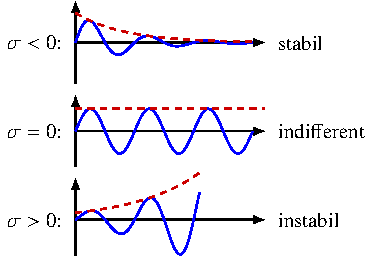
\includegraphics{papers/aircraft/images/eigenwerte.pdf}
    \caption{Verlauf der Lösung $e^{\lambda t}$ in den drei Fällen
    stabil ($\sigma < 0$), indifferent ($\sigma = 0$) und instabil ($\sigma > 0$).
    Die gestrichelte Kurve ist die Hüllkurve $e^{\sigma t}$.
    \label{aircraft:fig:eigenwerte}}
\end{figure}

Zwei Zeiten charakterisieren die Schwingung, die Periode $T$ und die
Halbwertszeit $t_{1/2}$.
Die \emph{Periode} (period) ist die Dauer einer vollen Schwingung.
Aus $\omega T = 2\pi$ folgt $T = 2\pi/\omega$.
Die \emph{Halbwertszeit} (time to half amplitude) ist die Zeit, nach der die
Hüllkurve $e^{\sigma t}$ auf die Hälfte gefallen ist.
Aus $e^{\sigma t_{1/2}} = \frac{1}{2}$ folgt
\begin{equation}
    t_{1/2}
    =
    -\frac{\ln 2}{\sigma}.
    \label{aircraft:eqn:halbwertszeit}
\end{equation}
Für $\sigma < 0$ ist die Halbwertszeit positiv und gibt an, wie rasch eine
Störung abklingt.
Für $\sigma > 0$ ist die Halbwertszeit negativ, denn die Hüllkurve fällt nie auf
die Hälfte, sondern wächst.
Der Betrag $|t_{1/2}| = \ln 2/\sigma$ ist dann die Zeit, in der die Hüllkurve
auf das Doppelte anwächst.
Diese Zeit heisst \emph{Verdoppelungszeit} (time to double amplitude).
Je grösser die Verdoppelungszeit ist, desto schwächer ist die Instabilität.
Entsprechend ist die Stabilität umso schwächer, je grösser die Halbwertszeit
ist.
Eine grosse Verdoppelungszeit lässt dem Piloten viel Zeit, eine Störung von
Hand zu korrigieren.

Die allgemeine Lösung der Bewegungsgleichung ist eine
Linearkombination der vier Lösungen $\vec{x}_0^{(k)} e^{\lambda_k t}$,
und die Störung legt die Anteile fest.

\subsection{Das komplexe Eigenwertpaar der Dutch Roll
\label{aircraft:subsection:eigenwertpaar}}
Die Systemmatrix ist reell, also treten komplexe Eigenwerte als
konjugierte Paare $\sigma \pm i\omega$ auf.
Die beiden Lösungen eines Paars setzen sich nach
Kapitel~\ref{chapter:differentialgleichungen} zur reellen Schwingung
$e^{\sigma t}\cos\omega t$ zusammen.
Ein reeller Eigenwert beschreibt eine Bewegung ohne Schwingung, ein
komplexes Paar eine Schwingung mit der Dämpfung $\sigma$ und der
Frequenz $\omega$.
Die Dutch Roll ist ein komplexes Eigenwertpaar.
Sie klingt genau dann ab, wenn $\sigma < 0$ ist.

\subsection{Die Eigenvektoren
\label{aircraft:section:5-eigenvektoren}}
Bisher haben wir nur die Eigenwerte gedeutet.
Die Lösung \eqref{aircraft:eqn:exponentialansatz} enthält aber auch den
Eigenvektor $\vec x_0$.
Der Eigenvektor ist ein Zustand, der sich unter dem Bewegungsgesetz nur um
den Faktor $e^{\lambda t}$ verändert.
Die Verhältnisse seiner vier Komponenten bleiben also erhalten.
Die Komponenten geben deshalb an, mit welcher Amplitude der Schiebewinkel, die
Rollrate, die Gierrate und der Rollwinkel an der Lösung beteiligt sind.
Eine Lösung $\vec x_0 e^{\lambda t}$ heisst \emph{Eigenbewegung} (mode).
Bei einem komplexen Eigenwert $\lambda$ hat die Gleichung
\eqref{aircraft:eqn:eigenwertgleichung-homogen} komplexe Koeffizienten, und der
Eigenvektor ist deshalb ebenfalls komplex.
Für den Vergleich der Komponenten verwenden wir dann ihre Beträge.

Am Eigenvektor lässt sich ablesen, welche Zustandsgrössen eine Eigenbewegung
betrifft.
Ist eine Komponente von $\vec x_0$ gross und sind die übrigen klein, so
betrifft die Eigenbewegung fast nur eine Zustandsgrösse.
Sind alle Komponenten von vergleichbarer Grösse, so sind alle Zustandsgrössen
beteiligt, und die Eigenbewegung ist gekoppelt im Sinne von
Abschnitt~\ref{aircraft:section:2-dynamisches-system}.
Wäre die Systemmatrix $A$ eine Diagonalmatrix, so wären die Eigenvektoren die
Einheitsvektoren, und keine Eigenbewegung wäre gekoppelt.
% (c) 2026 Stephanie Märklin, OST Ostschweizer Fachhochschule
%
% !TEX root = ../../buch.tex
% !TEX encoding = UTF-8
%
% Rolle im Paper: Beleg
%
\section{Rechenbeispiel und Vergleich realer Flugzeuge
\label{aircraft:section:6-rechenbeispiel}}
\kopfrechts{Rechenbeispiel}
In diesem Abschnitt wenden wir die Rechnung auf zwei reale Flugzeuge an, ein
einmotoriges Propellerflugzeug und einen Business Jet.
Für beide setzen wir die Derivative aus der Literatur ein und berechnen
Eigenwerte und Eigenvektoren.
Nach Abschnitt~\ref{aircraft:section:5-interpretation} lassen sich
Stabilität und Abklingzeit an den Eigenwerten ablesen.
Der Vergleich zeigt, wie sich zwei Konstruktionen in ihren Eigenwerten
unterscheiden, und damit in ihrer Stabilität.

\subsection{Das Propellerflugzeug
\label{aircraft:section:6-propellerflugzeug}}
Wir betrachten ein einmotoriges Propellerflugzeug im Horizontalflug.
Die Derivative für diesen Flugzustand stammen aus
Nelson~\cite[Tabelle 5.2 und Anhang B]{aircraft:nelson}.
Die Systemmatrix lautet damit
\begin{equation}
    A
    =
    \begin{pmatrix}
        -0.254 &  0     & -1.0   & 0.182 \\
        -16.02  & -8.40  &  2.19  & 0     \\
        4.488 & -0.350 & -0.760 & 0     \\
        0     &  1     &  0     & 0
    \end{pmatrix}.
    \label{aircraft:eqn:systemmatrix-ga}
\end{equation}
Die Nullstellen der charakteristischen Gleichung berechnen wir numerisch mit
MATLAB.
Das ergibt die vier Eigenwerte und ihre Halbwertszeiten nach
Gleichung~\eqref{aircraft:eqn:halbwertszeit},
\begin{align}
    \lambda_1     &= -8.433,              & t_{1/2} &= 0.08\,\text{s},
    \notag \\
    \lambda_2     &= -0.00891,            & t_{1/2} &= 78\,\text{s},
    \notag \\
    \lambda_{3,4} &= -0.486 \pm 2.334\,i, & t_{1/2} &= 1.4\,\text{s},
    \quad T = 2.7\,\text{s}.
    \label{aircraft:eqn:eigenwerte-ga}
\end{align}
Sie stimmen bis auf Rundungsunterschiede in den Derivativen mit den von
Nelson~\cite[Beispiel 5.3]{aircraft:nelson} angegebenen Werten überein.
Zwei Eigenwerte sind reell, zwei bilden ein komplexes Paar.
Nach Abschnitt~\ref{aircraft:section:5-eigenvektoren} besteht die
Seitenbewegung dieses Flugzeugs also aus zwei Eigenbewegungen ohne Schwingung
und einer Schwingung.

Welche Bewegungsform zu welchem Eigenwert gehört, lesen wir nach
Abschnitt~\ref{aircraft:section:5-eigenvektoren} an den Eigenvektoren ab.
Ein Eigenvektor ist nach Abschnitt~\ref{aircraft:section:4-eigenwerte} nur bis
auf einen Faktor bestimmt.
Wir teilen deshalb jeden Eigenvektor durch seine betragsgrösste Komponente,
so dass diese den Wert $1$ hat und die übrigen als Anteile davon erscheinen.
Die Tabelle~\ref{aircraft:table:eigenvektoren-ga} enthält die Beträge dieser
Komponenten.
Beim Eigenwert $\lambda_1$ sind nur die Rollrate und der Rollwinkel
nennenswert, beides Grössen der Längsachse, diese Eigenbewegung ist die
Rollbewegung.
Beim Eigenwert $\lambda_2$ dominiert der Rollwinkel, begleitet von einer
kleinen Gierrate, das ist das langsame Kippen mit Kursänderung der
Spiralbewegung.
Beim Paar $\lambda_{3,4}$ sind alle vier Komponenten von derselben
Grössenordnung.
Damit ist diese Eigenbewegung gekoppelt im Sinne von
Abschnitt~\ref{aircraft:section:system}, das ist die Dutch Roll.
Die drei Eigenbewegungen sind genau die drei Bewegungsformen aus
Abschnitt~\ref{aircraft:section:1-grundbegriffe}.

Mit der Zuordnung lassen sich die Halbwertszeiten aus
Gleichung~\eqref{aircraft:eqn:eigenwerte-ga} deuten.
Die Rollbewegung ist nach einer Zehntelsekunde auf die Hälfte abgeklungen.
Die Spiralbewegung braucht dafür über eine Minute und verläuft nach
Nelson~\cite[Abschnitt 5.1]{aircraft:nelson} so allmählich, dass der Pilot
sie nicht bewusst wahrnimmt.
Die Dutch Roll ist nach etwa einer halben Periode auf die Hälfte abgeklungen.
Alle vier Realteile sind negativ.
Die Seitenbewegung dieses Flugzeugs ist nach
Abschnitt~\ref{aircraft:section:5-interpretation} also stabil.
Damit ist die Frage aus Abschnitt~\ref{aircraft:section:1-grundbegriffe}
für dieses Flugzeug beantwortet.
Es kehrt in die Ruhelage zurück, und die Halbwertszeiten geben an, wie
schnell.

\begin{table}
    \centering
    \begin{tabular}{llrrrr}
        \hline
        Eigenwert & Bewegungsform & $|\beta|$ & $|p|$ & $|r|$ & $|\varphi|$ \\
        \hline
        $\lambda_1 = -8.433$                  & Rollbewegung
        & $0.008$ & $1.000$ & $0.041$ & $0.119$ \\
        $\lambda_2 = -0.00891$                & Spiralbewegung
        & $0.029$ & $0.009$ & $0.175$ & $1.000$ \\
        $\lambda_{3,4} = -0.486 \pm 2.334\,i$ & Dutch Roll
        & $0.454$ & $0.890$ & $1.000$ & $0.374$ \\
        \hline
    \end{tabular}
    \caption{Beträge der Eigenvektorkomponenten des Propellerflugzeugs,
        normiert auf die grösste Komponente, und die daraus abgelesene
        Bewegungsform.
        \label{aircraft:table:eigenvektoren-ga}}
\end{table}

\subsection{Der Business Jet
\label{aircraft:section:6-businessjet}}
Für den Business Jet gibt
Stengel~\cite[Lecture 20, Supplemental Material]{aircraft:stengel} die
Systemmatrix an, mit den Zustandsgrössen in der Reihenfolge $r$, $\beta$,
$p$, $\varphi$.
In der Reihenfolge von Gleichung~\eqref{aircraft:eqn:zustandsvektor}
umgeordnet lautet sie
\begin{equation}
    A
    =
    \begin{pmatrix}
        -0.1567 &  0      & -1      & 0.0958 \\
        -2.408  & -1.1616 &  0.2501 & 0      \\
        1.9011 &  0.0566 & -0.1079 & 0      \\
        0      &  1      &  0      & 0
    \end{pmatrix}.
    \label{aircraft:eqn:systemmatrix-bizjet}
\end{equation}
Dieselbe Rechnung wie beim Propellerflugzeug ergibt
\begin{align}
    \lambda_1     &= -1.203,              & t_{1/2} &= 0.6\,\text{s},
    \notag \\
    \lambda_2     &= +0.00883,            & t_{1/2} &= -78\,\text{s},
    \notag \\
    \lambda_{3,4} &= -0.116 \pm 1.390\,i, & t_{1/2} &= 6.0\,\text{s},
    \quad T = 4.5\,\text{s}.
    \label{aircraft:eqn:eigenwerte-bizjet}
\end{align}

Auch hier sind zwei Eigenwerte reell und zwei bilden ein Paar, und die
Eigenvektoren in Tabelle~\ref{aircraft:table:eigenvektoren-bizjet} zeigen
dieselbe Zuordnung wie beim Propellerflugzeug.
Bei der Rollbewegung ist der Rollwinkel grösser als beim Propellerflugzeug,
weil die Drehung langsamer abklingt und sich dabei mehr Rollwinkel ansammelt.

Die Rollbewegung klingt langsamer ab als beim Propellerflugzeug, aber immer
noch rasch.
Der Eigenwert der Spiralbewegung ist positiv, die Seitenbewegung dieses
Flugzeugs ist also instabil.
Die negative Halbwertszeit ist nach
Abschnitt~\ref{aircraft:section:5-interpretation} eine Verdoppelungszeit
von $78$\,s.
Eine Störung braucht über eine Minute, um sich zu verdoppeln.
Nelson~\cite[Tabelle 5.4]{aircraft:nelson} verlangt für gute
Flugeigenschaften eine Verdoppelungszeit von mindestens $20$\,s, ein
Pilot korrigiert diese Spiralbewegung also nebenbei.
Damit ist die Aussage aus Abschnitt~\ref{aircraft:section:1-grundbegriffe}
bestätigt, dass die Spiralbewegung leicht korrigierbar ist.
Die Dutch Roll ist stabil, braucht aber mehr als eine Periode, bis sie auf
die Hälfte abgeklungen ist, beim Propellerflugzeug reicht dafür eine halbe
Periode.

\begin{table}
    \centering
    \begin{tabular}{llrrrr}
        \hline
        Eigenwert & Bewegungsform & $|\beta|$ & $|p|$ & $|r|$ & $|\varphi|$ \\
        \hline
        $\lambda_1 = -1.203$                  & Rollbewegung   & $0.010$
        & $1.000$ & $0.069$ & $0.831$ \\
        $\lambda_2 = +0.00883$                & Spiralbewegung & $0.006$
        & $0.009$ & $0.095$ & $1.000$ \\
        $\lambda_{3,4} = -0.116 \pm 1.390\,i$ & Dutch Roll     & $0.718$
        & $1.000$ & $0.954$ & $0.717$ \\
        \hline
    \end{tabular}
    \caption{Beträge der Eigenvektorkomponenten des Business Jets,
        normiert auf die grösste Komponente, und die daraus abgelesene
        Bewegungsform.
        \label{aircraft:table:eigenvektoren-bizjet}}
\end{table}

\subsection{Vergleich
\label{aircraft:section:6-vergleich}}
Die Tabelle~\ref{aircraft:table:vergleich} stellt Dämpfung, Frequenz,
Periode und Halbwertszeit der drei Bewegungsformen beider Flugzeuge
gegenüber.
Die Abbildung~\ref{aircraft:fig:komplexe-ebene} zeigt die Eigenwerte in der
komplexen Ebene.
Der Abstand eines Eigenwerts von der imaginären Achse ist seine Dämpfung,
sein Abstand von der reellen Achse seine Frequenz.
Beide Flugzeuge haben dieselben drei Bewegungsformen, die Eigenwerte liegen
aber an verschiedenen Stellen.
Die Rollbewegung des Propellerflugzeugs liegt weit links, die des Business
Jets nahe bei den anderen Eigenwerten.
Die beiden Spiralbewegungen liegen fast am selben Ort, aber auf
verschiedenen Seiten der imaginären Achse, und das entscheidet über die
Stabilität.
Die Dutch Roll des Business Jets liegt näher bei der imaginären Achse als
die des Propellerflugzeugs, sie ist schwächer gedämpft.
Die Stabilität und die Abklingzeiten beider Flugzeuge lassen sich damit
vollständig aus der Lage der Eigenwerte ablesen.

\begin{table}
    \centering
    \begin{tabular}{llrrrr}
        \hline
        Flugzeug & Bewegungsform
        & $\sigma$ & $\omega$ & $T$ [s] & $t_{1/2}$ [s] \\
        \hline
        Propellerflugzeug & Rollbewegung
        & $-8.433$           & --      & --    & $0.08$ \\
        & Spiralbewegung
        & $-0.00891$         & --      & --    & $78$   \\
        & Dutch Roll
        & $-0.486$           & $2.334$ & $2.7$ & $1.4$  \\
        \hline
        Business Jet      & Rollbewegung
        & $-1.203$           & --      & --    & $0.6$  \\
        & Spiralbewegung
        & $+0.00883$         & --      & --    & $-78$  \\
        & Dutch Roll
        & $-0.116$           & $1.390$ & $4.5$ & $6.0$  \\
        \hline
    \end{tabular}
    \caption{Dämpfung, Frequenz, Periode und Halbwertszeit der drei
    Bewegungsformen beider Flugzeuge.
    Die negative Halbwertszeit der Spiralbewegung des Business Jets ist eine
    Verdoppelungszeit.
    \label{aircraft:table:vergleich}}
\end{table}

\begin{figure}
    \centering
    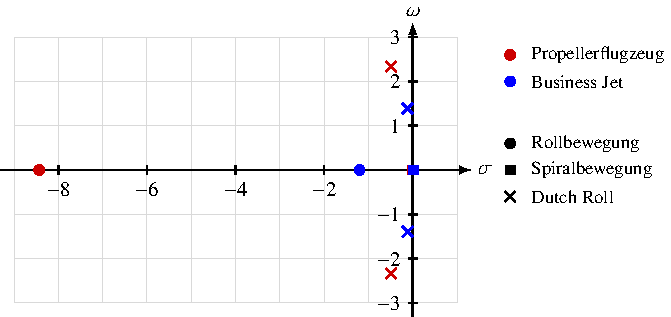
\includegraphics{papers/aircraft/images/komplexe-ebene.pdf}
    \caption{Eigenwerte des Propellerflugzeugs und des Business Jets in
    der komplexen Ebene.
    Die Farbe unterscheidet die Flugzeuge, der Marker die Bewegungsform.
    Die Eigenwerte der beiden Spiralbewegungen liegen bei $-0.009$ und
        $+0.009$ und sind in dieser Skala nicht zu unterscheiden.
        \label{aircraft:fig:komplexe-ebene}}
\end{figure}



%
% 7-fluegel.tex -- Einfluss der Flügelgeometrie auf die Eigenwerte
%
% (c) 2026 Stephanie Märklin, OST Ostschweizer Fachhochschule
%
% !TEX root = ../../buch.tex
% !TEX encoding = UTF-8
%
\section{Einfluss der Flügelgeometrie auf die Eigenwerte
\label{aircraft:section:fluegel}}
\kopfrechts{Flügelgeometrie}
Die Systemmatrizen des Propellerflugzeugs und des Business Jets in
Abschnitt~\ref{aircraft:section:6-beispiel} haben dieselbe Form.
Die beiden Flugzeuge unterscheiden sich nur in den Werten der Derivative.
Diese Werte entstehen aus der Geometrie des Flugzeugs.
Wir betrachten die drei Derivative $L_\beta$, $N_\beta$ und $N_r$.
Diese drei bestimmen die Spiralbewegung und die Dutch Roll, und der
Konstrukteur legt sie über die Form der Flügel und des Seitenleitwerks fest.

Die \emph{V-Form} (dihedral) ist der Winkel, um den die Flügel gegenüber der
Querachse nach oben geneigt sind.
Schiebt das Flugzeug, so trifft die Luft den Flügel auf der Seite, zu der das
Flugzeug schiebt, unter einem grösseren Anstellwinkel als den anderen Flügel.
Dieser Flügel erzeugt mehr Auftrieb, und das Flugzeug rollt von dieser Seite
weg.
Dieses Rollmoment infolge Schiebens ist das Derivativ $L_\beta$ aus
Abschnitt~\ref{aircraft:section:system}.
Mit wachsender V-Form wächst der Betrag von $L_\beta$.

Die \emph{Pfeilung} (sweep) ist der Winkel, um den die Flügel gegenüber der
Querachse nach hinten geneigt sind.
Beim Schieben steht der Flügel auf der Seite, zu der das Flugzeug schiebt,
weniger schräg zur Anströmung als der andere Flügel und erzeugt ebenfalls mehr
Auftrieb.
Die Pfeilung vergrössert den Betrag von $L_\beta$ ebenso wie die V-Form.

Das \emph{Seitenleitwerk} (vertical tail) bestimmt die beiden
Derivative $N_\beta$ und $N_r$.
Schiebt das Flugzeug, so wird das Seitenleitwerk schräg angeströmt und erzeugt
ein Giermoment, das die Nase in die Anströmung dreht.
Dieses Giermoment infolge Schiebens ist die Richtungsstabilität $N_\beta$.
Giert das Flugzeug, so bewegt sich das Seitenleitwerk quer zur Flugrichtung und
erzeugt ein Giermoment gegen die Drehung.
Dieses Giermoment infolge Gierens ist die Gierdämpfung $N_r$.
Ein grösseres Seitenleitwerk vergrössert die Beträge von $N_\beta$ und $N_r$
zugleich.
Die Dutch Roll wird begünstigt, wenn der Betrag von $L_\beta$ gross ist im
Vergleich zu $N_\beta$.

Wie die Derivative die Eigenwerte festlegen, zeigt die Spiralbewegung am
einfachsten, denn ihr Eigenwert ist reell und lässt sich näherungsweise in
geschlossener Form angeben.
Nelson \cite{aircraft:nelson} gibt die Näherung
\begin{equation}
    \lambda_{\text{S}}
    \approx
    \frac{L_\beta N_r - L_r N_\beta}{L_\beta}
    \label{aircraft:eqn:spiralnaeherung}
\end{equation}
an, wobei $L_r$ das Rollmoment infolge Gierens ist.
Bei üblichen Vorzeichen sind $L_\beta$ und $N_r$ negativ, $L_r$ und $N_\beta$
positiv.
Der Nenner ist also negativ, und der Eigenwert der Spiralbewegung ist genau dann
negativ, wenn
\begin{equation}
    L_\beta N_r - L_r N_\beta > 0
    \label{aircraft:eqn:spiralbedingung}
\end{equation}
gilt.
Tatsächlich ist für das Propellerflugzeug mit den Werten aus Nelson Tabelle~5.2
\[
    L_\beta N_r - L_r N_\beta
    =
    (-16{,}02)\cdot(-0{,}76) - 2{,}19\cdot 4{,}49
    =
    12{,}18 - 9{,}83
    >
    0.
\]
Der Eigenwert der Spiralbewegung ist nach
Abschnitt~\ref{aircraft:section:6-beispiel} negativ, wie es die Bedingung
verlangt.
Die Bedingung \eqref{aircraft:eqn:spiralbedingung} wird umso leichter erfüllt,
je grösser die Beträge von $L_\beta$ und $N_r$ sind.
Ob die Spiralbewegung abklingt oder anwächst, entscheidet das Verhältnis der
vier Derivative und damit die Konstruktion.

Nelsons Näherung für die Dutch Roll vernachlässigt die Rollbewegung und enthält
$L_\beta$ deshalb nicht.
Nelson \cite[Abb.~5.14]{aircraft:nelson} zeigt stattdessen, wie die Eigenwerte
in der komplexen Ebene wandern, wenn der Betrag von $L_\beta$ wächst.
Der Eigenwert der Spiralbewegung wandert nach links, das Eigenwertpaar der
Dutch Roll wandert nach rechts.
Eine grosse V-Form stabilisiert die Spiralbewegung und schwächt die Dämpfung der
Dutch Roll.
Eine grosse Richtungsstabilität $N_\beta$ wirkt umgekehrt, denn sie erhöht die
Frequenz der Dutch Roll und zieht den Eigenwert der Spiralbewegung zum Ursprung.
Der Konstrukteur muss beide Eigenwerte zugleich in der linken Halbebene halten.
Die Gierdämpfung $N_r$ vergrössert die Dämpfung beider Bewegungen, lässt sich
durch ein grösseres Seitenleitwerk aber nur zusammen mit $N_\beta$ vergrössern.

Der Vergleich in Abschnitt~\ref{aircraft:section:6-beispiel} ist mit diesem
Zusammenhang verträglich.
Der Business Jet hat gepfeilte Flügel, das Propellerflugzeug gerade.
Die Dutch Roll des Business Jets ist mit $\sigma = -0{,}116$ schwächer gedämpft
als die des Propellerflugzeugs mit $\sigma = -0{,}487$.

Die Geometrie legt die Derivative fest, und die Derivative legen die
Eigenwerte fest.
Ob ein Flugzeug stabil ist, wird damit beim Entwurf entschieden.
%
% 8-grenzen.tex -- Grenzen des Modells und aktive Dämpfung
%
% (c) 2026 Stephanie Märklin, OST Ostschweizer Fachhochschule
%
% !TEX root = ../../buch.tex
% !TEX encoding = UTF-8
%
% Rolle im Paper: Gültigkeitsbereich
% Roter Faden: Nur kleine Störungen, ein Flugzustand pro A,
% ausgeblendete Kopplung zur Spiralmode, Yaw Damper.
% Überleitung aus dem vorangehenden Abschnitt: Gilt das uneingeschränkt?
%
\section{Grenzen des Modells und aktive Dämpfung
\label{aircraft:section:grenzen}}
\kopfrechts{Grenzen des Modells}
Das Bewegungsgesetz gilt nach Abschnitt~\ref{aircraft:section:system} nur für
kleine Störungen um die Ruhelage.
Bei grossen Auslenkungen hängen die Kräfte und Momente nicht mehr linear von den
Zustandsgrössen ab, und die Derivative sind keine Konstanten mehr.
Bei hohen Anstellwinkeln kann die Rolldämpfung $L_p$ ihr Vorzeichen wechseln und
positiv werden \cite{aircraft:stengel}.
Die Rollbewegung, die nach Abschnitt~\ref{aircraft:section:1-grundbegriffe} bei
gewöhnlichen Anstellwinkeln rasch abklingt, wächst dann an.
Das lineare Modell sagt dieses Verhalten nicht voraus, weil es mit den
Derivativen der Ruhelage rechnet.

Die Werte in der Systemmatrix gelten für ein Flugzeug in einem Flugzustand.
Eine andere Geschwindigkeit, eine andere Höhe oder eine andere Klappenstellung
ergibt andere Derivative und damit andere Eigenwerte.
Ein Flugzeug muss das Stabilitätskriterium in jedem Flugzustand erfüllen, den
es erreicht.
Die Rechnung aus Abschnitt~\ref{aircraft:section:4-eigenwerte} ist deshalb für
jeden Flugzustand zu wiederholen.
Dabei kann sich auch die Art der Eigenwerte ändern.
Der Fall zweier komplexer Eigenwertpaare tritt ein, wenn Rollbewegung und
Spiralbewegung zu einer gemeinsamen Schwingung verschmelzen, wie
Stengel \cite{aircraft:stengel} am Versuchsflugzeug M2-F2 zeigt.

Wir haben uns in Abschnitt~\ref{aircraft:section:system} auf die
Seitenbewegung beschränkt und die Längsbewegung ausgeblendet.
Für kleine Störungen ist das gerechtfertigt, weil die beiden Bewegungen dann
voneinander unabhängig sind.
Bei schnellen Rollmanövern und bei hohen Anstellwinkeln koppeln Trägheitskräfte
und aerodynamische Kräfte die Seitenbewegung mit der Längsbewegung
\cite{aircraft:nelson}.
Diese Fälle liegen ausserhalb des Modells.

Liefert die Geometrie nicht genügend Dämpfung, so wird die Dämpfung künstlich
erzeugt.
Ein \emph{Gierdämpfer} (yaw damper) ist ein automatisches System, das die
Gierrate $r$ misst und das Seitenruder proportional dazu ausschlägt, so dass
das Ruder der Drehung entgegenwirkt \cite{aircraft:nelson}.
Das zusätzliche Giermoment ist proportional zu $r$ und wirkt in der
Systemmatrix wie eine grössere Gierdämpfung $N_r$.
Nach Abschnitt~\ref{aircraft:section:fluegel} verschiebt ein grösserer Betrag
von $N_r$ das Eigenwertpaar der Dutch Roll nach links.
In der Sprache von Abschnitt~\ref{aircraft:subsection:realteil} wird der
Realteil $\sigma$ kleiner, und die Störung klingt schneller ab.
Diese Rückkopplung einer gemessenen Grösse auf ein Ruder heisst
\emph{Stabilitätsaugmentation} (stability augmentation) und verändert die
Einträge der Systemmatrix durch Regelung \cite{aircraft:nelson}.
Die meisten Verkehrsflugzeuge sind mit einem Gierdämpfer ausgerüstet
\cite{aircraft:nelson}.
Ein Verkehrsflugzeug muss auch bei Ausfall des Gierdämpfers fliegbar bleiben,
und der Konstrukteur berechnet deshalb die Eigenwerte der ungeregelten und der
geregelten Systemmatrix.

Bei Kampfflugzeugen wird die Stabilität zugunsten der Wendigkeit meist
deutlich reduziert.
\cite{aircraft:sadraey}.
Für ein solches Flugzeug ist die Stabilitätsaugmentation keine Verbesserung,
sondern die Bedingung dafür, dass es fliegbar ist.
Ein \emph{automatisches Flugregelsystem} (automatic flight control system)
steuert die Ruder durchgehend.
Der Gierdämpfer verändert einen Eintrag der Systemmatrix, das
automatische Flugregelsystem verändert mehrere Einträge zugleich.
Über die Stabilität eines solchen Flugzeugs entscheiden die Eigenwerte der
geregelten Systemmatrix.
%
% 9-fazit.tex -- Komplexe Eigenwerte als Entwurfswerkzeug
%
% (c) 2026 Stephanie Märklin, OST Ostschweizer Fachhochschule
%
% !TEX root = ../../buch.tex
% !TEX encoding = UTF-8
%
% Rolle im Paper: Fazit
% Roter Faden: Das dynamische Verhalten steckt in wenigen komplexen Zahlen,
% anwendbar im Entwurf statt im Flugversuch.
% Überleitung aus dem vorangehenden Abschnitt: Was bleibt als Ergebnis?
%
\section{Komplexe Eigenwerte als Entwurfswerkzeug
\label{aircraft:section:fazit}}
\kopfrechts{Entwurfswerkzeug}
Die Leitfrage lautet, warum wir die Stabilität eines Flugzeugs berechnen
müssen und wie wir es können.
Berechnen müssen wir die Stabilität, weil die Beobachtung im Flug erst möglich
ist, wenn das Flugzeug existiert, und weil die Beobachtung kein Mass für die
Stabilität liefert (Abschnitt~\ref{aircraft:section:3-mathematische-stabilitaet}).
Berechnen können wir die Stabilität, weil die Seitenbewegung für kleine
Störungen dem linearen Bewegungsgesetz \eqref{aircraft:eqn:bewegungsgesetz}
folgt.
Stabilität bedeutet in diesem Modell, dass jede Lösung abklingt
(Abschnitt~\ref{aircraft:section:3-mathematische-stabilitaet}).

Der Exponentialansatz \eqref{aircraft:eqn:ansatz} führt das Bewegungsgesetz
auf die Eigenwertgleichung \eqref{aircraft:eqn:eigenwertgleichung} zurück.
Die Eigenwerte sind die Nullstellen der charakteristischen Gleichung
\eqref{aircraft:eqn:charakteristisch}.
Der Realteil eines Eigenwerts entscheidet nach
Abschnitt~\ref{aircraft:section:5-interpretation}, ob die zugehörige Bewegung
abklingt, der Imaginärteil, ob sie schwingt.
Halbwertszeit \eqref{aircraft:eqn:halbwertszeit} und Periode übersetzen die
Eigenwerte in Zeiten, die der Pilot im Flug wahrnimmt.
Das dynamische Verhalten der Seitenbewegung ist damit durch vier komplexe
Zahlen bestimmt.

Die Derivative in der Systemmatrix liegen aus der Geometrie vor, bevor das
Flugzeug fliegt (Abschnitt~\ref{aircraft:subsection:systemmatrix}).
Die Eigenwerte lassen sich deshalb im Entwurf berechnen und mit den
Anforderungen an die Flugeigenschaften vergleichen.
Die Anforderungen, die Nelson \cite{aircraft:nelson} in Tabelle~5.4
wiedergibt, verlangen für Flugzeuge mittleren Gewichts eine Verdopplungszeit
der Spiralbewegung von mindestens $20$\,s.
Der Business Jet aus Abschnitt~\ref{aircraft:section:6-beispiel} erfüllt diese
Anforderung mit $78$\,s, obwohl seine Spiralbewegung instabil ist.
Genügt ein Entwurf den Anforderungen nicht, so zeigt
Abschnitt~\ref{aircraft:section:fluegel}, welche Derivative zu verändern sind,
und Abschnitt~\ref{aircraft:section:grenzen}, wie ein Gierdämpfer die Dämpfung
künstlich erhöht.
Die Frage, ob ein Flugzeug stabil ist, beantworten wir damit, bevor das
Flugzeug gebaut ist.




\printbibliography[heading=subbibliography]
\end{refsection}
